\documentclass{beamer}
\usepackage{graphicx}

\setbeameroption{show notes on second screen=bottom}
\title[Embedding of DDL]{Deep embedding of Dyadic Deontic Logic in Isabelle}
\subtitle{Bachelor Semester 2 project}
\author[Hlushakov]{Illia Hlushakov}
\institute[Unilux BiCS]{Bachelor in Computer Science\\Univertait Letzebuerg}

\begin{document}
\maketitle

\begin{frame}
\tableofcontents
\end{frame}

\section{Dyadic Deontic Logic}

\subsection{Syntax}
\begin{frame}{Deontic elements}

\begin{block}{Conditional obligation}
	$$\bigcirc(\psi/\varphi)$$
	Is interepreted as "Obliged to $\psi$, given that $\phi$"
\end{block}
	
\begin{block}{Settled state}
	$$\square\varphi$$
	Is interepreted as "$\varphi$ is settled to be", meaning it is true in every possibility
\end{block}	
\end{frame}

\begin{frame}{BNF of DDL}
	\begin{block}{Minimal syntax}
	$$\varphi = \varphi\ |\ \neg\varphi\ |\ \psi \to \varphi\ |\ \square \psi\ |\ \bigcirc(\psi/\varphi)$$
	\end{block}

	\begin{block}{Full syntax}
	$$\varphi\lor\psi \equiv \neg\varphi \to \psi$$
	$$\varphi\land\psi \equiv \neg(\varphi \to \neg\psi)$$
	$$\diamond\varphi \equiv \neg\square\neg\varphi$$
	$$P(\psi/\varphi) \equiv \neg\bigcirc(\neg\psi/\varphi)$$
	\end{block}
\end{frame}

\subsection{Semantics}

\begin{frame}{Preference semantics}
	\begin{block}{Model of semantics}
	$$M = \langle W,\succeq, V\rangle$$
	The model of preference is a triplet of the set of non-empty worlds $W$, beterness relation $\succeq$ on the world set and a valuation function $V: W \to \mathcal{P}(W)$. The betterness relation contains information about which worlds are bettern then another. 
	\end{block}
\end{frame}

\begin{frame}{Relation properties}
There are variants of preferance models, which correspond to different proof systems

	\begin{itemize}
	\item Class of preferance models, where R is any relation
	\item Class of preferance models, where R is reflexive and transitive
	\item Class of preferance models, where R is total
	\item Class of preferance models, where R is reflexive, transitive and total
	\end{itemize}
\end{frame}


\begin{frame}{Formal semantics}
$$M,w \vDash p \text{ iff } w \in V(p)$$
$$M,w \vDash \neg\phi \text{ iff } M,w \nvDash \phi$$
$$M,w \vDash \varphi \to \psi \text{ iff } M,w \vDash \varphi \to M,w \vDash \psi $$
$$M,w \vDash \square\varphi \text{ iff } \forall t \in W, M,t \vDash \varphi \in V(p)$$
$$M,w \vDash \bigcirc(\psi/\varphi) \text{ iff } \text{best}(\|\varphi\|) \subset \|\psi\|$$
\end{frame}

\begin{frame}{Deep and shallow embeddings}
The Deep embedding approach is to introduce the logic as new types, and functions on them. Contrary, the shallow approach is to represent the logic as formulas inside HOL, with existing types of i, bool and functions between them.
I will compare my deep embedding with Shallow embedding of Parent and Benzmüller.
\end{frame}

\subsection{Embedding of propositions}
\begin{frame}{Propositions in deep an shallow}
	\begin{block}{Propositions in shallow}
		\begin{figure}
		\centering
		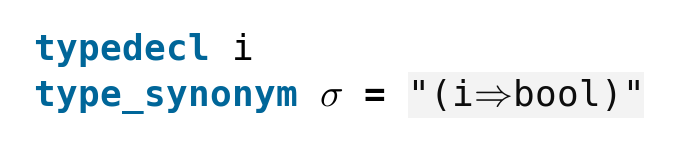
\includegraphics[width=0.5\textwidth]{resources/ShallowPrimTypes.png}
		\end{figure}
	In shallow embedding, only a type of the worlds is used, \texttt{i}. Propositions are mappings from type of worlds to type of booleans.
	\end{block}
	\begin{block}{Prospositions in deep}
		\begin{figure}
		\centering
		
\includegraphics[width=0.25\textwidth]{resources/DeepPrimTypes.png}
		\end{figure}
	In deep embedding, the type of world also exists, but also a type of atomic propositions. Thus atomic propositions are a primitive type, not a type derived from others.  
	\end{block}
\end{frame}

\subsection{Embedding of syntax}
\begin{frame}{Syntax of shallow embedding}
	\begin{figure}
	\centering
	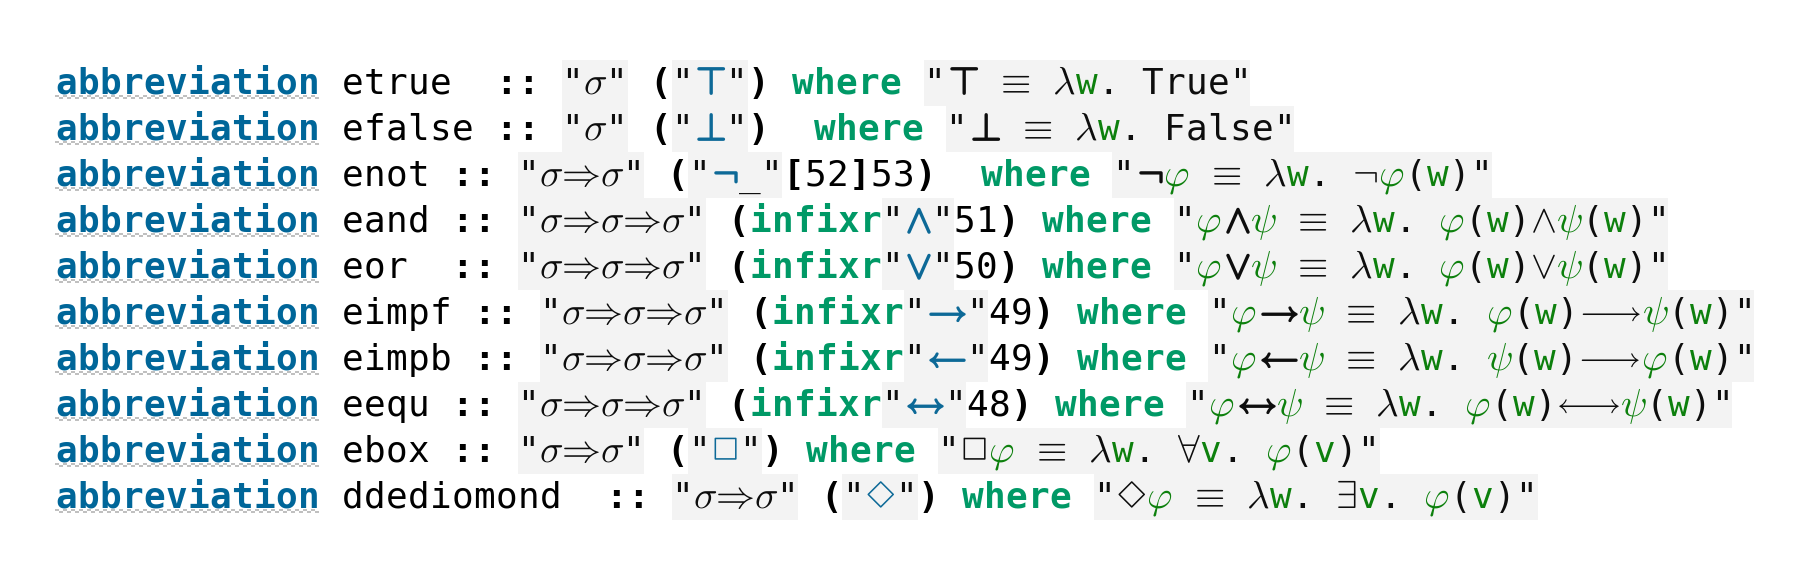
\includegraphics[width=0.8\textwidth]{resources/ShallowSyntax.png}
	\end{figure}
In the shallow embedding, the syntax represents formulas within HOL. In all cases, the logical connectives are lambda abstractions, that feed the world to the underlying propositions and then perform
\end{frame}

\begin{frame}{Syntax of deep embedding}
	\begin{figure}
	\centering
	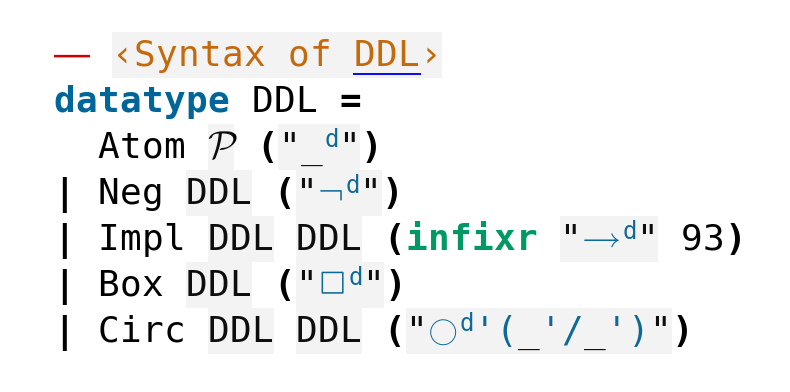
\includegraphics[width=0.8\textwidth]{resources/DeepSyntax.png}
	\end{figure}
	In the deep embeding, the syntax is represented as new type, called \texttt{DDL}, elements of whose are the formulas in the language. The new type is defined using \texttt{datatype} feature, which creates a new type elemnts of whose are closed under given relations/contructors. \note{A datatype is embedded with in HOL, as an initial algebra for the functor, that is defined from the consutrctors: An empty constructor corresponds to unit type, a contructor with other types corresponds to cartesian product of these types.}
	Each constructor represents a part of the language: atomic propositions, negation, implication, settled state, and conditional obligation 
\end{frame}

\subsection{Embedding of semantics}
\begin{frame}{Semantics in shallow embedding}
	\begin{figure}
	\centering
	
\includegraphics[width=\textwidth]{resources/ShallowValidity.png}
	\end{figure}
	The semantics is get by the fact, that every proposition already knows its value at that world. The satisfability is embedded in the definition of proposition, and thus validity is as simple as requring that the world is satisfiable in one formula. 	
\end{frame}

\begin{frame}{Semantics in deep embedding}
	\begin{figure}
	\centering
	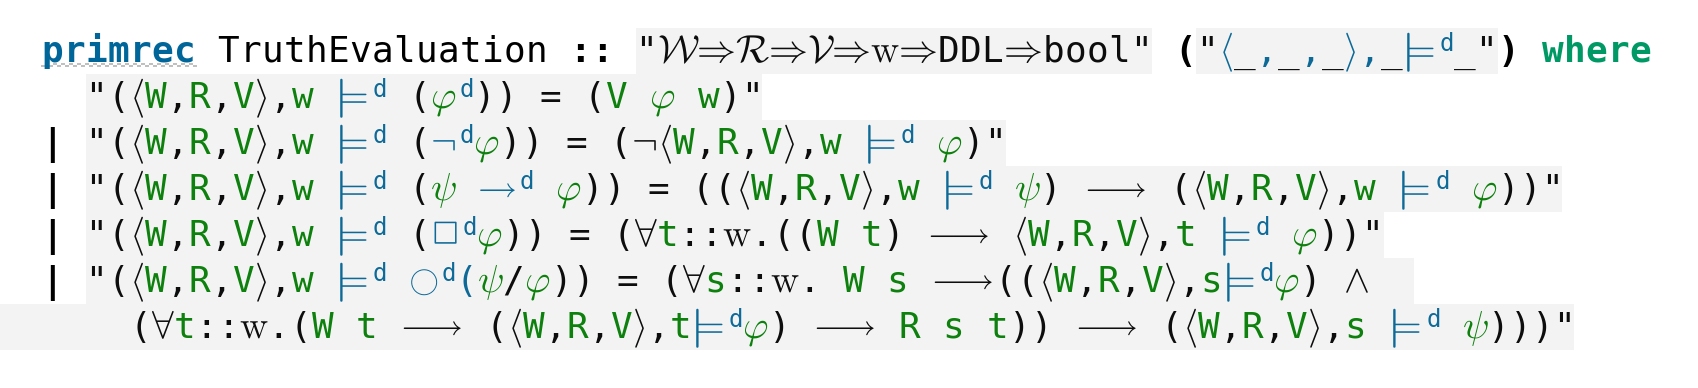
\includegraphics[width=0.8\textwidth]{resources/DeepSat.png}
	\end{figure}
The semantics of deep embedding consits of valuation function, and then the validity definition, with a frame condition.
\end{frame}

\begin{frame}{Disecting deontic evaluation}
	\begin{figure}
	\centering
	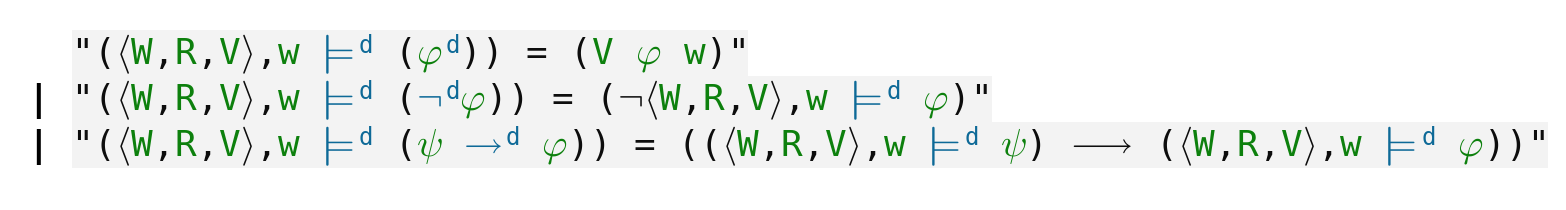
\includegraphics[width=\textwidth]{resources/StdValidCases.png}
	\end{figure}
\end{frame}
\begin{frame}{Disecting deontic evaluation}
	\begin{figure}
	\centering
	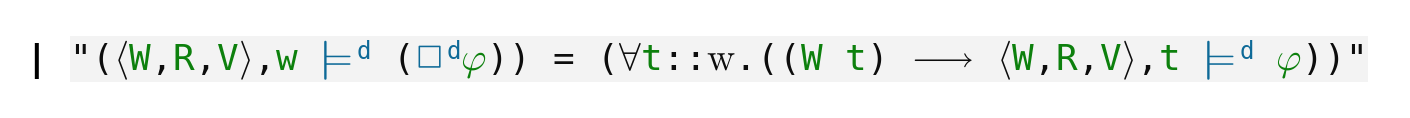
\includegraphics[width=\textwidth]{resources/SqValidCase.png}
	\end{figure}
\end{frame}
\begin{frame}{Disecting deontic evaluation}
	\begin{figure}
	\centering
	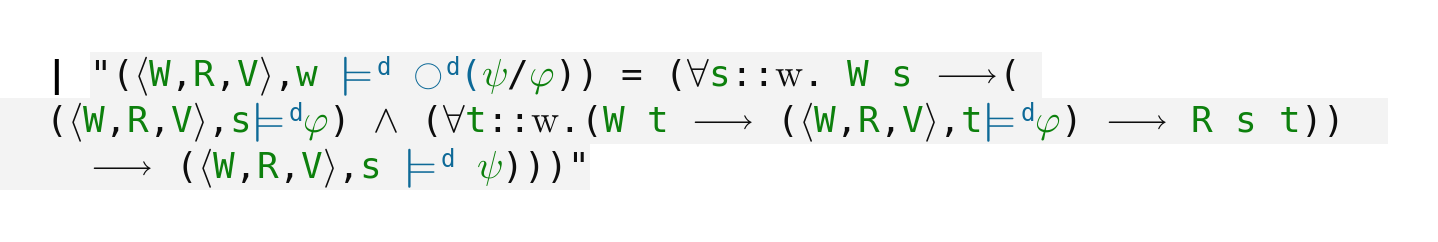
\includegraphics[width=\textwidth]{resources/ObValidCase.png}
	\end{figure}
\end{frame}
\begin{frame}{Disecting deontic validity}
	\begin{figure}
	\centering
	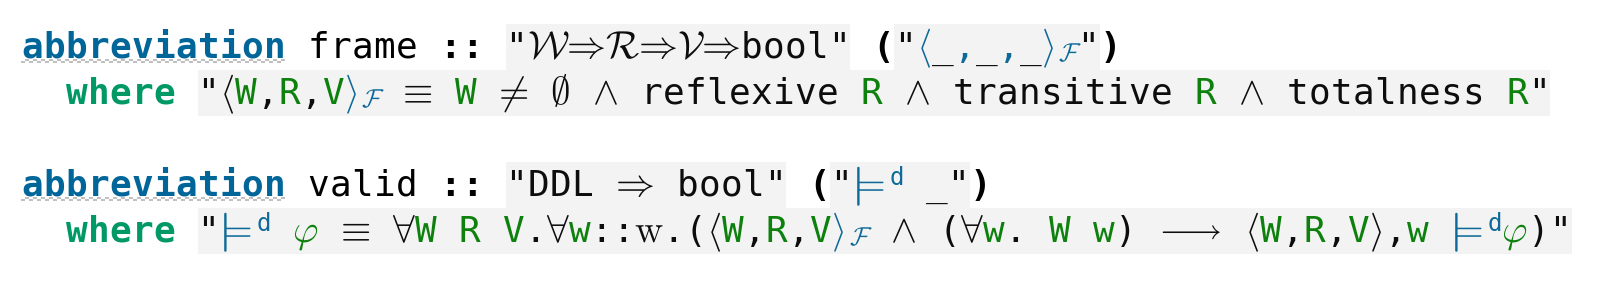
\includegraphics[width=\textwidth]{resources/DeepValidity.png}
	\end{figure}
\end{frame}



\subsection{Embedding of proof system}
\begin{frame}{Proof system inside Shallow}
	\begin{figure}
	\centering
	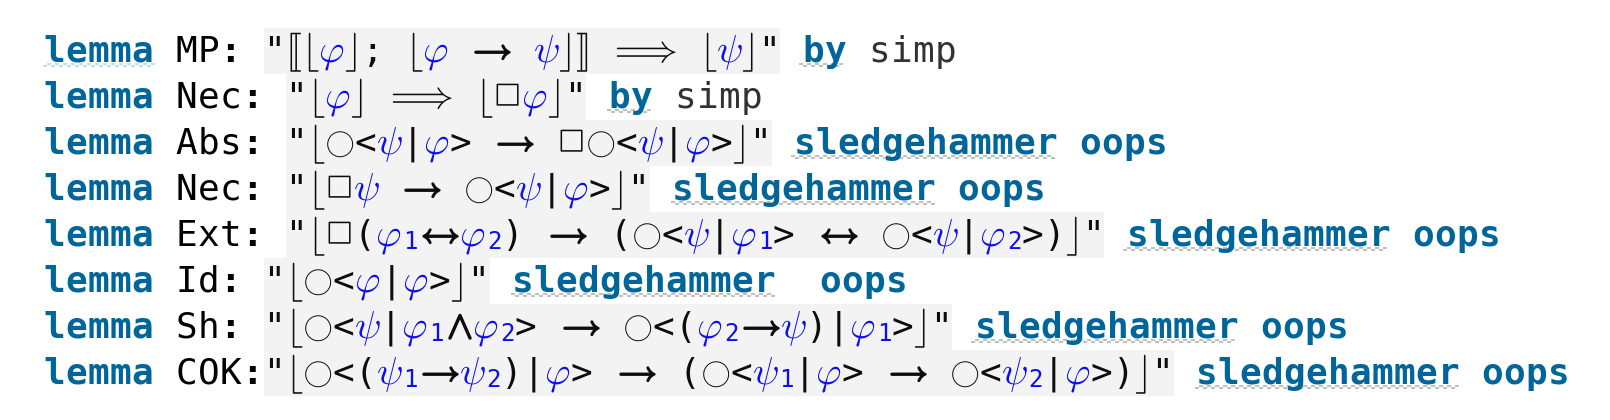
\includegraphics[width=0.8\textwidth]{resources/ShallowProofSystem.png}
	\end{figure}
In the shallow embedding, the proof system is not implemented, but rather it is shown that it lies inside the semantics, with the addition of relational properties, thus showing the correspondance between properties of the relation and the proof system the semantics satisfy.
\end{frame}

\begin{frame}{Proof system in deep embedding}
	\begin{figure}
	\centering
	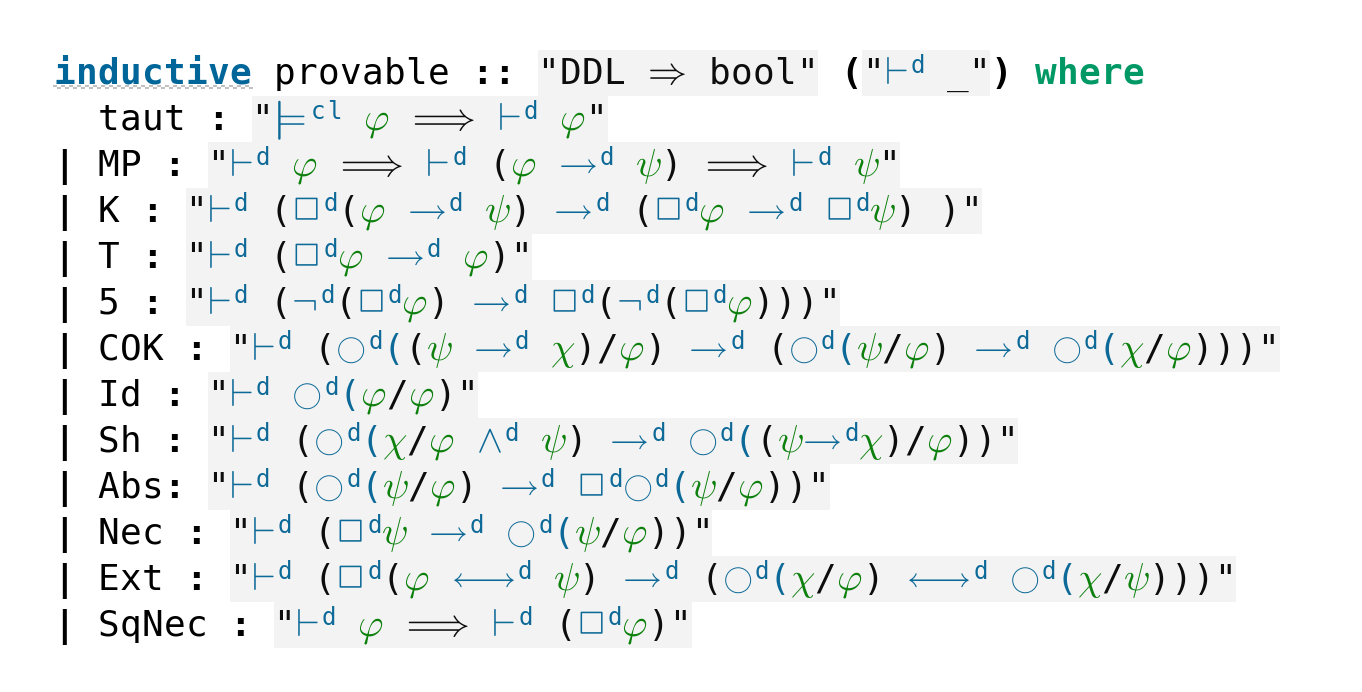
\includegraphics[width=0.8\textwidth]{resources/DeepProofSystem.png}
	\end{figure}
I have decided to implement proof system fully as a separated definition, rather than simply lemmas, to embody the nature of the proof system. It is simplemented as an inductive defition \texttt{provable}. If a formulas is provable, is can be contructed from the axiom schemas, using rule schemas. \note{An inductive definition is the least set that is closed under certain relations. In this case, it is the set of all axiom schemas,  that are closed under modem ponens and nesciation} 
\end{frame}

\section{Soundness proof}
\begin{frame}{Soundness}
A proof system is sound, if every provable formula is valid, i.e.
$$\vdash \varphi \Longrightarrow \vDash \varphi$$
Worth to note, that the semantics can have different frame conditions (reflexivity, transivity and totalness). I have managed to show, that the Aqvist's proof system is sound for semantics without any frame condition, and for semantics with reflexivity, transivity and totalness.
\end{frame}

\begin{frame}{Proof}
The proof was primeraly a structural induction on the provable definition. Most cases where solved easly, by mere evaluation of the formulas. Most of them were easly found by Sledgehammer. However, the tatology case was requiring some attention:
$$\vDash^{\text{cl}} \varphi \Longrightarrow \vDash^\text{d} \varphi$$
In this case, a solution was to use a special wrapper $\lambda \psi. \langle W,R,V\rangle,w \vDash^d \psi$, as a bridge between classical valuation via a valuation function and deontic evaluation
\end{frame}

\begin{frame}{Classical valuation}
	\begin{figure}
	\centering
	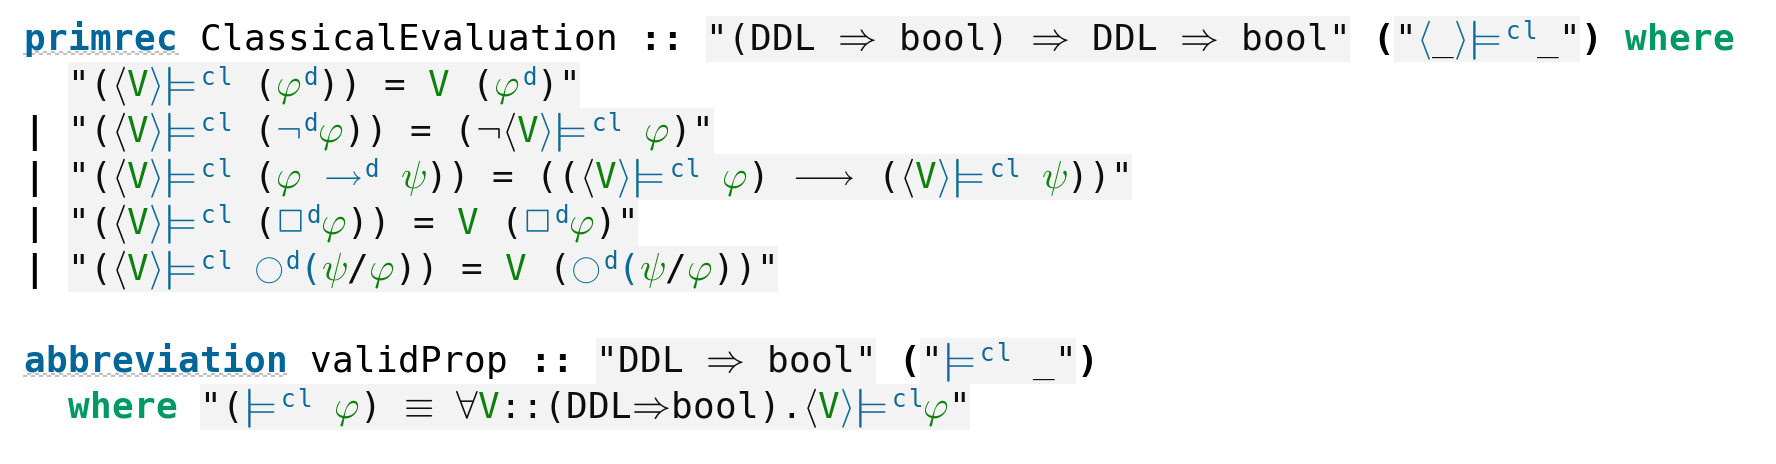
\includegraphics[width=0.8\textwidth]{resources/ClassicalValuation.png}
	\end{figure}
The classical evaluation is implmeneted, with the deontic formulas treated as classical, "opaque" formulas
\end{frame}

\section{Conclusion}
\begin{frame}{To conclude}
	\begin{itemize}
	\item I have deeply embedded dyadic deontic logic in HOL
	\item I have shown that proof system is sound, for both classes of all preference models and preference models with reflexive, transitive, total relations.
	\end{itemize}
\end{frame}

\begin{frame}
\centering
Thank you for your attention. Any questions?
\end{frame}
\end{document}




